\chapter{A Data Overview}
\label{ch_data_overview}

\begin{center}
  \textit{With insufficient data it is easy to go wrong.}

 - Carl Sagan
\end{center}

NMR data can be broadly grouped into four categories based on when it
is known.  First, Figure \ref{data_overview_1}, 
there is information that is known without performing
any NMR experiments: this includes information about the molecule as well
as general NMR and molecular knowledge.  Second,
Figure \ref{data_overview_2}, is data that is 
collected using the NMR spectrometer, and is known before analysis begins.  
Third, Figure \ref{data_overview_3}, is the information generated during 
analysis, and fourth, Figure \ref{data_overview_4}, is the final goal of 
an NMR study, information about the actual structure of the molecule of 
interest.

This chapter will present the data generated during the NMR process.
Later chapters will focus in on subsets of the data, as well as show how
the data is used during analysis.


\section{Global prior knowledge}
Knowledge of NMR and molecules that is available before any experiments are
performed.

\subsection*{Molecule}

\subsubsection{Primary sequence}
The primary sequence of amino acids of the protein is known. For example, the 
sequence of Ubiquitin is 
MQIFVKTLTG KTITLEVEPS DTIENVKAKI QDKEGIPPDQ QRLIFAGKQL EDGRTLSDYN IQKESTLHLV LRLRGG
according to Swiss-Prot.

\subsubsection{Amino acids}
The atoms contained in each amino acid (see Table \ref{alanine_atoms}), 
bond lengths between atom pairs (see Table \ref{alanine_bond_lengths}), 
and bond angles (see Table \ref{alanine_bond_angles}) are known 
\cite{alanine_sreepad}.

\subsection*{NMR}

\subsubsection{Nuclei}
The gyromagnetic ratio of nuclei (see Table \ref{gyromagnetic_ratios}) and 
pulse sequences.  The gyromagnetic ratio and the magnetic field strength 
determine the approximate frequency range at which nuclei appear in spectra.

\subsubsection{Time-domain data}
Resonances appear as decaying sinusoids, and the full data set is a sum of
many of those sinusoids at various frequencies and intensities.

\subsubsection{Through-bond experiments}
Time-domain free induction decay (FID)s are collected using
pulse sequences \cite{khaneja2005} designed to target specific nuclei by
exploiting the coupling constants and characteristic chemical shifts of specific 
nuclei and functional groups.  The collected FIDs are sums of decaying sinusoids.

The pulse sequence determines which covalently bound groups will appear in 
experiments (see Tables \ref{nhsqc_peaktypes}, \ref{hnco_peaktypes}, 
\ref{hncacb_peaktypes}, \ref{hbhaconh_peaktypes}, \ref{cconh_peaktypes}, and
\ref{hcconh_peaktypes}).

\subsubsection{Through-space experiments}
Nuclear Overhauser Effect (NOE) \cite{noe_kaiser} experiments transfer 
magnetization between spatially near proton pairs, and do not require a 
network of covalent bonds.  Each true peak indicates a pair of protons within 
approximately 5 Angstroms of each other.  This is different from 
through-bond correlation spectra, in which peaks indicate the nuclei of covalently 
bonded atoms; NOESY spectra depend not on covalent bonds but rather 
on spatial proximity.  Thus, each NOESY peak contains some information 
about the actual three-dimensional structure of a molecule, although this
information is not used until the correspondence between peak cross
section and an atom's nucleus is determined.

\subsubsection{Resonance}
A particular nucleus is expected to resonate at approximately the same 
frequency in all spectra (although factors such as temperature and the 
Bloch-Siegert shift can produce differences).

\subsubsection{Frequency-domain spectra}
The Fourier Transform of a decaying sinusoid produces a frequency-domain 
spectrum with a peak at a frequency matching the oscillation frequency of 
the sinusoid.  Since NMR time-domain data consists of multiple decaying 
sinusoids caused by nuclei resonating at characteristic chemical shifts, 
the frequency domain spectrum will contain peaks for every oscillating 
sinusoid present in the time-domain data.  

Spectra contain peaks, which are characterized to obtain volume and peak
cross section attributes; peak cross sections are characterized to obtain 
position and width attributes (see Figure \ref{peak_1d}).

\subsubsection{Chemical shift statistics}
Statistics from previously analyzed molecules are maintained by the BMRB
\cite{bmrb}, which show clear trends of average chemical shifts based on
both amino acid type and nucleus (see Table \ref{alanine_atoms} for the 
chemical shift statistics of alanine).

Chemical shift values are correlated to secondary structure, as described
by secondary chemical shift statistics \cite{spera1991empirical}.  Chemical 
shifts are also correlated to three-dimensional structure, as shown by 
CHESHIRE \cite{cheshire} and CS-ROSETTA \cite{cs-rosetta}.  


\section{Local prior knowledge}
Knowledge which is available after performing NMR experiments, but before
performing analysis.

\subsection*{Sample}

\subsubsection{Preparation procedure}
The procedure used to express and purify a sample of interest, including
growth medium and conditions, expression organism, and buffer optimization.

\subsubsection{Isotope labeling}
The specific H, N, and C labeling pattern.  While \nmrisoh{} is 
the most abundant isotopye of hydrogen, and convenient for NMR experiments,
\nmrisoc{} is the most abundant isotope of carbon and is not 
NMR-active; \textsuperscript{2}H is not as easy to observe because of
its nuclear spin value of 1 (as opposed to the proton's spin value of 1/2),
but can improve the quality of experiments observing nearby protons because,
in comparison to protons, nearby nuclei are afforded fewer relaxation pathways.
Labeling patterns with specific properties have been implemented to take
advantage of these different properties, as in SAIL-FLYA \cite{sail_flya}.
See Table \ref{gyromagnetic_ratios}.

\subsubsection{Sample contents}
The components present in the sample as well as their concentrations.
Samples can degrade and aggregate over time, and may be affected by the
NMR experiments.

\subsection*{NMR}

\subsubsection{Spectrometer}
Operating characteristics of the spectrometer, such as its field strength.

\subsubsection{Time-domain data}
The experimental conditions in which each time-domain data set is collected, 
its sampling schedule, and the FIDs themselves.

For each time-domain data set, the delay between data points, number of 
points collected, and total delay between the first and last point (or 
acquisition time, which may be calculated from the first two parameters).

The sample schedule gives rise to frequency-domain artifacts according to 
its point spread function, and also determines which means can be used to
process the time-domain data to frequency-domain.  Two examples of different
types of sample schedule are shown in Figure \ref{schedule_uniform} and
Figure \ref{schedule_nonuniform}.

\subsubsection{Spectra}
The set of frequency-domain spectra and the spectral processing workflow
used to construct them.  Key attributes are the spectral width, or range of
different frequencies that can be distinguished, and resolution, or the
ability to distinguish nearby but distinct signals in the frequency domain
\cite{ernst2004}.  See Figure \ref{nhsqc} for an example Nitrogen 
Heteronuclear Single-Quantum Coherence (HSQC) spectrum.

\subsubsection{Stereospecific ambiguities}
Given the set of spectra collected, the atoms in the molecule, and the isotope
labeling scheme, there may be stereospecifically ambiguous assignments.  See
Table \ref{stereospecific_ambiguities} for a list of potential ambiguities.



\section{Analysis}
Knowledge which is obtained while analyzing the experimentally collected data.

This includes peak picking (see Figure \ref{nhsqc_peaks} for a peak picked spectrum), 
the assembly of peaks into GSSs, GSS and resonance typing, sequential
GSS assignments, and sequence-specific GSS assignments.
In general, the correspondence between resonances, which appear in NMR spectra 
as peak cross sections, and atomic nuclei is not known.  The correspondence 
between resonances and peak cross sections is also not known, and is difficult 
to determine in the presence of ambiguity.

GSSs \cite{saga, ezassign, pistachio, autoassign1997, autoassign2001}
and resonances \cite{ccpn} correspond to residues and nuclei.
They are key to data analysis because they link the data collected in NMR
experiments to the molecular details of the sample.
Although these concepts had been used to a limited extent by earlier programs
such as XEasy and Sparky \cite{xeasy, sparky}, more recent work has treated 
GSSs and resonances as explicit, first-class members of data analysis 
\cite{ccpn, bmrb}.  These definitions are based on the BMRB and CCPN data models,
the complete documentation of the NMR-STAR data dictionary may be found online 
at \url{http://www.bmrb.wisc.edu/dictionary/} and
\url{http://www.ccpn.ac.uk/software/extras/datamodelfolder/datamodel}.
% also \url{http://www2.ccpn.ac.uk/api-documentation/}. 
% also \url{http://www2.ccpn.ac.uk/api-documentation/ccpnmr/ccpnmr2.2/python/doc/api.html}
% also \url{http://www2.ccpn.ac.uk/api-documentation/ccpnmr/ccpnmr2.2/model/doc/ccp/nmr/index.html}

\subsection*{Peak}
A feature of a spectrum that corresponds to a group of covalently bound
resonances (in a through-bond spectrum) or to a pair of nearby protons
(in a NOESY spectrum).  A peak has one cross section
for each dimension of the spectrum in which it appears; each cross section
corresponds to a resonance at a characteristic frequency.

\subsection*{Resonance}
A resonance is an NMR-visible signal which corresponds to a nucleus \cite{ccpn}.
In general, a nucleus resonates at a single characteristic frequency based
on its local environment;  a resonance will be found at the same 
frequency across multiple experiments.  This phenomenon is used to aid in 
identification, although it is confounded by degeneracy as well as proteins
with multiple conformations.

A resonance is used to link a peak cross section to a nucleus, for a chemical 
shift assignment, by means of a spin system and a residue.  Each peak cross 
section is assigned a resonance, and the resonances are assigned to spin 
systems, with the semantics that they are covalently bound.

\subsection*{Generic spin system}
A generic spin system (GSS) is an NMR-visible group of peaks, typically 
across multiple spectra, which corresponds to a group of covalently bonded 
resonances; it is similar to a residue.  
The key to GSSs is a set of multi-dimensional pulse 
sequences designed to correlate resonances within GSSs 
\cite{cavanagh1995protein, hncacb, hnco, cbcaconh}, which are
based on an N-H group (due to its sensitivity and chemical shift dispersion)
and correlate additional nearby nuclei through covalent bonds.

These pulse sequences use several types of overlap.  First, each
includes the N-H group.  Second, due to the similar scalar couplings between
N and the CA and CA(i-1) nuclei, it is possible to simultaneously correlate an
N-H group with both nearby CA nuclei; this means that each CA may be correlated
with two N-H groups, or in other words, may be a part of two H-N-rooted GSSs. 
Third, due to the scalar coupling between N and CO(i-1), correlations to 
C*(i-1) appear in two pulse sequences of a pair (e.g. HNCACB and CBCA(CO)NH), 
while C* appear in only the HNCACB.  See Figure \ref{ccpn_nhsqc}, 
Figure \ref{ccpn_hncacb}, Figure \ref{ccpn_cbcaconh}, Figure \ref{ccpn_hnco}, 
Figure \ref{ccpn_hncaco}, Figure \ref{ccpn_cconhtocsy}, Figure \ref{ccpn_hcchtocsy},
Figure \ref{ccpn_hcconhtocsy}, and Figure \ref{ccpn_hbhaconh} for an 
illustration of the correlated nuclei.  Table \ref{pulse_sequences} tabulates
the number of distinct measurements of each nucleus that can be obtained from
common pulse sequences under ideal conditions.

These characteristics lead to a definition of a GSS: a root 
resonance or resonances, typically an amide H-N group, and additional 
covalently-bonded resonances.  The precise extent of a GSS is in principle 
determined by the available NMR experiments \cite{hncacb, hnco, cbcaconh}.  
In practice, a backbone GSS often is initially 
comprised of a backbone H-N, CO, CA, CB, CO(i-1), CA(i-1), and CB(i-1).

\subsubsection{Sidechain GSSs}
The standard pulse sequences can also excite sidechain resonances, if the 
chemical shifts of the resonances and the coupling constants between those
resonances are similar to those of the targeted backbone resonances.
Typically, sidechain GSSs are observed for tryptophan, asparagine, glutamine,
and arginine residues in H-N-rooted pulse sequences.
The potential GSS types for common pulse sequence are given in Tables 
\ref{nhsqc_peaktypes}, \ref{hnco_peaktypes}, 
\ref{hncacb_peaktypes}, \ref{hbhaconh_peaktypes}, \ref{cconh_peaktypes}, and
\ref{hcconh_peaktypes}.



\section{Desired knowledge}

\subsection*{Restraints}
Through the analysis process, structural constraints are obtained.  These 
constraints include H-H interatomic distances obtained from NOESY spectra
(see Figure \ref{structure_restraints}), residual dipolar couplings (RDCs) 
(see Figure \ref{structure_restraints}) which give orientation constraints
between two nuclei, and torsion angles (see Figure \ref{torsion_angles}) 
which constrain the orientation of three adjacent bonds. In structural 
models, constraints that are not satisfied. are known as "violations".

\subsection*{Structure} 
The three-dimensional coordinates of the atoms, or correspondingly, the
three-bond torsion angles.  Either of these describes the molecular structure.



\clearpage
\section{Tables}

\begin{table}[h]
  \begin{tabular}{ | c | c | }
    \hline
    Atom name   &  Average chemical shift (PPM) of nucleus \\  \hline
    C           &  187.20     \\  \hline
    O           &  --         \\  \hline
    N           &  123.32     \\  \hline
    H           &  8.19       \\  \hline
    HA          &  4.25       \\  \hline
    CA          &  53.16      \\  \hline
    HB1         &  1.35       \\  \hline
    HB2         &  1.35       \\  \hline    
    HB3         &  1.35       \\  \hline
    CB          &  19.06      \\  \hline
  \end{tabular}
  \caption[The atomic nuclei in alanine, in a protein chain.]
          {The atomic nuclei in alanine, in a protein chain.
           Average chemical shift statistics are taken from the BMRB.}
  \label{alanine_atoms}
\end{table}

\begin{table}
  \begin{tabular}{ | c | c | c | }
    \hline
    Atom 1  &   Atom 2  &  length (Angstroms)   \\  \hline
    C   &   N   &   1.45  \\  \hline
    C   &   C   &   1.51  \\  \hline
    C   &   O   &   1.25  \\  \hline
    N   &   H   &   1.03  \\  \hline
    C   &   H   &   1.1   \\  \hline
    O   &   H   &   1.1   \\  \hline
  \end{tabular}
  \caption[Alanine bond lengths, calculated from first principles.]
          {Alanine bond lengths, calculated from first principles
           in \cite{alanine_sreepad}.}
  \label{alanine_bond_lengths}
\end{table}

\begin{table}
  \begin{tabular}{ | c | c | c | c | }
    \hline
    Atom 1  &   Atom 2  &  Atom 3  &  estimated angle (degrees)   \\  \hline
    C   &   CA  &   CB  &   128  \\  \hline
    C   &   CA  &   N   &   112  \\  \hline
    N   &   CA  &   CB  &   110  \\  \hline
    O   &   C   &   CA  &   120  \\  \hline
  \end{tabular}
  \caption[Estimates of alanine bond angles.]
          {Estimates of alanine bond angles.  The first two are
           calculated from first priniciples in \cite{alanine_sreepad};
           the latter two are based on number of atoms bonded
           to the central atom.}
  \label{alanine_bond_angles}
\end{table}

\begin{table}
  \begin{tabular}{ | c | c | }
    \hline
    Nucleus &   gyromagnetic ratio (MHz / Tesla)  \\  \hline
    \textsuperscript{1}H    &   42.576  \\  \hline
    \textsuperscript{13}C   &   10.705  \\  \hline
    \textsuperscript{15}N   &   -4.316  \\  \hline
    \textsuperscript{19}F   &   40.052  \\  \hline
    \textsuperscript{31}P   &   17.235  \\  \hline
  \end{tabular}
  \caption{Gyromagnetic ratios of biologically important nuclei.}
  \label{gyromagnetic_ratios}
\end{table}

\begin{table}
  \begin{tabular}{ | c | c | }
    \hline
    Covalently-bound group       &  Amino acid sequence  \\  \hline
    H-N                          &  [\^{}P]              \\  \hline
    HE-NE                        &  R                    \\  \hline
    HD21-ND2                     &  N                    \\  \hline
    HD22-ND2                     &  N                    \\  \hline
    HE21-NE2                     &  Q                    \\  \hline
    HE22-NE2                     &  Q                    \\  \hline
    HE1-NE1                      &  W                    \\  \hline
  \end{tabular}
  \caption{The covalent groups that appear in the NHSQC experiment.}
  \label{nhsqc_peaktypes}
\end{table}

\begin{table}
  \begin{tabular}{ | c | c | }
    \hline
    Covalently-bound group       &  Amino acid sequence  \\  \hline
    H-N-C(i-1)                   &  .[\^{}P]             \\  \hline
    HE-NE-CZ                     &  R                    \\  \hline
    HD21-ND2-CG                  &  N                    \\  \hline
    HD22-ND2-CG                  &  N                    \\  \hline
    HE21-NE2-CD                  &  Q                    \\  \hline
    HE22-NE2-CD                  &  Q                    \\  \hline
    HE1-NE1-CE1                  &  W                    \\  \hline
  \end{tabular}
  \caption{The covalent groups that appear in the HNCO experiment.}
  \label{hnco_peaktypes}
\end{table}
    
\begin{table}
  \begin{tabular}{ | c | c | }
    \hline
    Covalently-bound group       &  Amino acid sequence  \\  \hline
    H-N-CA                       &  .[\^{}P]             \\  \hline
    H-N-CA(i-1)                  &  .[\^{}P]             \\  \hline
    H-N-CB                       &  .[\^{}PG]            \\  \hline
    H-N-CB(i-1)                  &  [\^{}G][\^{}P]       \\  \hline
    HE-NE-CD                     &  R                    \\  \hline
    HD21-ND2-CB                  &  N                    \\  \hline
    HD21-ND2-CA                  &  N                    \\  \hline
    HD22-ND2-CB                  &  N                    \\  \hline
    HD22-ND2-CA                  &  N                    \\  \hline
    HE21-NE2-CG                  &  Q                    \\  \hline
    HE21-NE2-CB                  &  Q                    \\  \hline
    HE22-NE2-CG                  &  Q                    \\  \hline
    HE22-NE2-CB                  &  Q                    \\  \hline
  \end{tabular}
  \caption{The covalent groups that appear in the HNCACB experiment.}
  \label{hncacb_peaktypes}
\end{table}

\begin{table}
  \begin{tabular}{ | c | c | }
    \hline
    Covalently-bound group       &  Amino acid sequence         \\  \hline
    H-N-HA(i-1)                  &  [\^{}G][\^{}P]              \\  \hline
    H-N-HA2(i-1)                 &  G[\^{}P]                    \\  \hline
    H-N-HA3(i-1)                 &  G[\^{}P]                    \\  \hline
    H-N-HB(i-1)                  &  [ITV][\^{}P]                \\  \hline
    H-N-QB(i-1)                  &  A[\^{}P]                    \\  \hline
    H-N-HB2(i-1)                 &  [PRNDCQEHLKMFSWY][\^{}P]    \\  \hline
    H-N-HB3(i-1)                 &  [PRNDCQEHLKMFSWY][\^{}P]    \\  \hline
  \end{tabular}
  \caption{The covalent groups that appear in the HBHA(CO)NH experiment.}
  \label{hbhaconh_peaktypes}
\end{table}

\begin{table}
  \begin{tabular}{ | c | c | }
    \hline
    Covalently-bound group              &  Amino acid sequence  \\  \hline
    H-N-C*(i-1), * in (A)               &  G[\^{}P]             \\  \hline
    H-N-C*(i-1), * in (A, B)            &  [HDSNCAFYW][\^{}P]   \\  \hline
    H-N-C*(i-1), * in (A, B, G)         &  [EQM][\^{}P]         \\  \hline
    H-N-C*(i-1), * in (A, B, G2)        &  T[\^{}P]             \\  \hline
    H-N-C*(i-1), * in (A, B, G, D)      &  [RP][\^{}P]          \\  \hline
    H-N-C*(i-1), * in (A, B, G1, G2)    &  V[\^{}P]             \\  \hline
    H-N-C*(i-1), * in (A, B, G, D, E)   &  K[\^{}P]             \\  \hline
    H-N-C*(i-1), * in (A, B, G1, G2, D1)&  I[\^{}P]             \\  \hline
    H-N-C*(i-1), * in (A, B, G, D1, D2) &  L[\^{}P]             \\  \hline
    % sidechain 
    HD21-ND2-C*, * in (B, A)            &  N (sidechain)            \\  \hline
    HD22-ND2-C*, * in (B, A)            &  N (sidechain)            \\  \hline
    HE21-NE2-C*, * in (G, B, A)         &  Q (sidechain)            \\  \hline
    HE22-NE2-C*, * in (G, B, A)         &  Q (sidechain)            \\  \hline
  \end{tabular}
  \caption{The covalent groups that appear in the C(CO)NH-TOCSY experiment.}
  \label{cconh_peaktypes}
\end{table}

\begin{table}
  \begin{tabular}{ | c | c | }
    \hline
    H-N-H*(i-1), * in A2, A3                          &  G[\^{}P]             \\  \hline
    H-N-H*(i-1), * in A, B2, B3                       &  [HDSNCFYW][\^{}P]    \\  \hline
    H-N-*(i-1), * in HA, QB                           &  A[\^{}P]             \\  \hline
    H-N-*(i-1), * in HA, HB, QG2                      &  T[\^{}P]             \\  \hline
    H-N-H*(i-1), * in A, B2, B3, G2, G3           &  [EQM][\^{}P]         \\  \hline
    H-N-H*(i-1), * in A, B2, B3, G2, G3, D2, D3       &  [RP][\^{}P]          \\  \hline
    H-N-*(i-1), * in HA, HB, QG1, QG2                 &  V[\^{}P]             \\  \hline
    H-N-H*(i-1), * in A, B2, B3, G3, G3, D2, D3, E2, E3   &  K[\^{}P] \\  \hline
    H-N-*(i-1), * in HA, HB, HG12, HG13, QG2, QD1     &  I[\^{}P]             \\  \hline
    H-N-*(i-1), * in HA, HB2, HB3, HG, QD1, QD2       &  L[\^{}P]             \\  \hline
    % sidechain
    HD21-ND2-*, * in (HB3, HB2, HA)   &  N (sidechain)                  \\  \hline
    HD22-ND2-*, * in (HB3, HB2, HA)   &  N (sidechain)                  \\  \hline
    HE21-NE2-*, * in (HG3, HG2, HB3, HB2, HA)   &  Q (sidechain)        \\  \hline
    HE22-NE2-*, * in (HG3, HG2, HB3, HB2, HA)   &  Q (sidechain)        \\  \hline
  \end{tabular}
  \caption{The covalent groups that appear in the HC(CO)NH-TOCSY experiment.}
  \label{hcconh_peaktypes}
\end{table}


\begin{table}
  \begin{tabular}{ | c | c | c |}
    \hline
    Ambiguity type     & Atomic nuclei &  Amino acid types     \\  \hline 
    3 nuclei, 1 peak   &  QB           &  A                    \\  \hline 
    3 nuclei, 1 peak   &  QG1          &  I                    \\  \hline 
    3 nuclei, 1 peak   &  QG2          &  [TI]                 \\  \hline 
    3 nuclei, 1 peak   &  QE           &  M                    \\  \hline 
    2 nuclei, 2 peaks  &  HA2/HA3      &  G                    \\  \hline 
    2 nuclei, 2 peaks  &  HB2/HB3      &  [RHKDESNQCPLMFYW]    \\  \hline 
    2 nuclei, 2 peaks  &  HG2/HG3      &  [RKEQPM]             \\  \hline 
    2 nuclei, 2 peaks  &  HG12/HG13    &  I                    \\  \hline 
    2 nuclei, 2 peaks  &  HD2/HD3      &  [RKP]                \\  \hline 
    2 nuclei, 2 peaks  &  HD21/HD22    &  N                    \\  \hline 
    2 nuclei, 2 peaks  &  HE2/HE3      &  K                    \\  \hline 
    2 nuclei, 2 peaks  &  HE21/HE22    &  Q                    \\  \hline 
    2 nuclei, 2 peaks  &  CG1/CG2      &  V                    \\  \hline 
    2 nuclei, 2 peaks  &  CD1/CD2      &  L                    \\  \hline 
    2 nuclei, 2 peaks or 2 nuclei, 1 peak  &  HD1/HD2  &  [YF]  \\  \hline 
    2 nuclei, 2 peaks or 2 nuclei, 1 peak  &  HE1/HE2  &  [YF]  \\  \hline 
    2 groups of 3 nuclei, 2 peaks  &  QG1/QG2  &  V            \\  \hline
    2 groups of 3 nuclei, 2 peaks  &  QD1/QD2  &  L            \\  \hline
  \end{tabular}
  \caption{Ambiguities in stereospecific assignments.}
  \label{stereospecific_ambiguities}
\end{table}

\begin{table}
    \begin{tabular}{ | c || c | c | c | c | c |}
    \hline
              & NHSQC & HNCO & HN(CA)CO & HNCACB & CBCA(CO)NH \\    \hline
      H       & 1     & 1    &        2 & 4      & 2     \\    \hline
      N       & 1     & 1    &        2 & 4      & 2     \\    \hline
      CO      & 0     & 1    &        0 & 0      & 0     \\    \hline
      CO(i-1) & 0     & 1    &        1 & 0      & 0     \\    \hline
      CA      & 0     & 0    &        0 & 1      & 0     \\    \hline
      CA(i-1) & 0     & 0    &        0 & 1      & 1     \\    \hline
      CB      & 0     & 0    &        0 & 1      & 0     \\    \hline
      CB(i-1) & 0     & 0    &        0 & 1      & 1     \\    \hline
    \end{tabular}
    \caption{The number of times nuclei typically appear in pulse sequences.}
    \label{pulse_sequences}
\end{table}


% figures
\clearpage
\section{Figures}

\begin{figure}[h]
  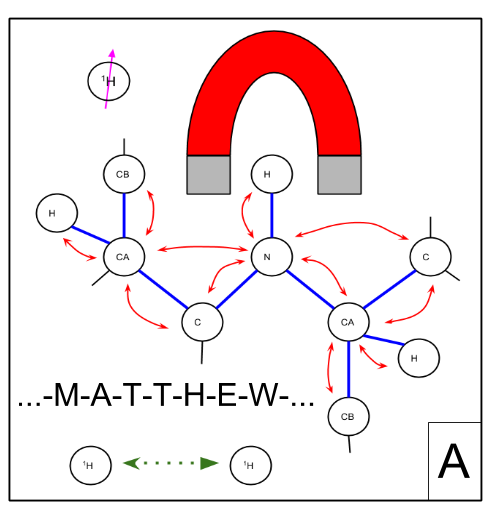
\includegraphics[scale=0.7]{figures/data_overview_1}
  \caption[General NMR and molecular knowledge.]
          {General NMR and molecular knowledge, including NMR phenomenon
           such as through-bond and through-space interactions, primary
           sequence, and gyromagnetic ratios.}
  \label{data_overview_1}
\end{figure}

\begin{figure}
  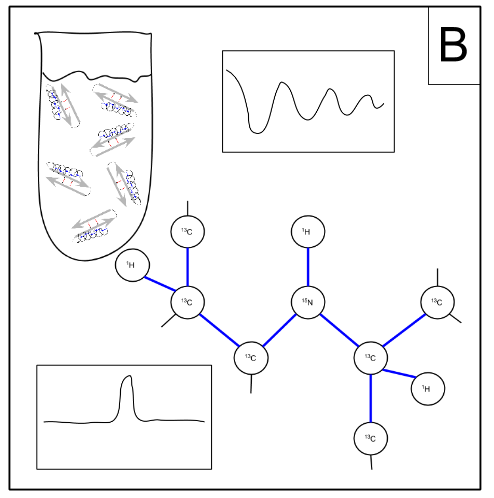
\includegraphics[scale=0.7]{figures/data_overview_2}
  \caption[Experimentally determined knowledge: obtained before analysis.]
          {Experimentally determined knowledge: obtained before analysis,
           including sample preparation and conditions, isotopic labeling,
           and time-domain and frequency-domain data.}
  \label{data_overview_2}
\end{figure}

\begin{figure}
  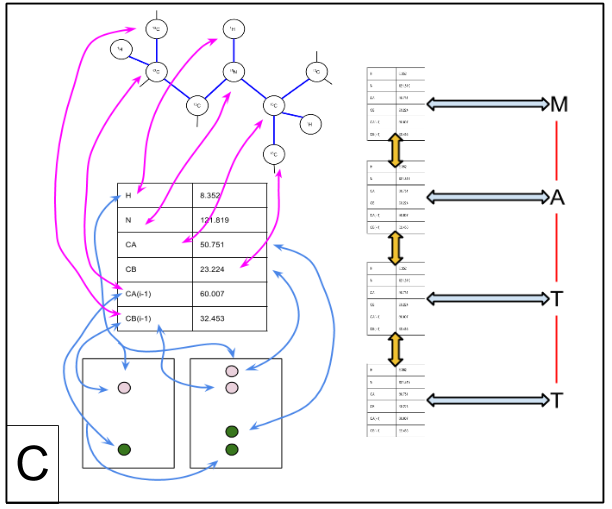
\includegraphics[scale=0.6]{figures/data_overview_3}
  \caption[Knowledge obtained during analysis.]
          {Knowledge obtained during analysis, including peaks, GSSs,
           resonances, sequential and sequence-specific assignments, and
           chemical shifts.}
  \label{data_overview_3}
\end{figure}

\begin{figure}
  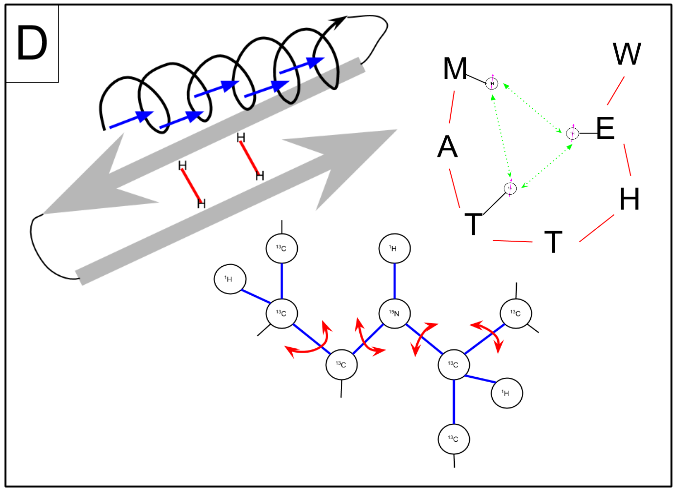
\includegraphics[scale=0.5]{figures/data_overview_4}
  \caption[Information about the actual physical properties of a molecule.]
          {Information about the actual physical properties of a molecule
           is derived from structural and angle restraints.}
  \label{data_overview_4}
\end{figure}

\begin{figure}
  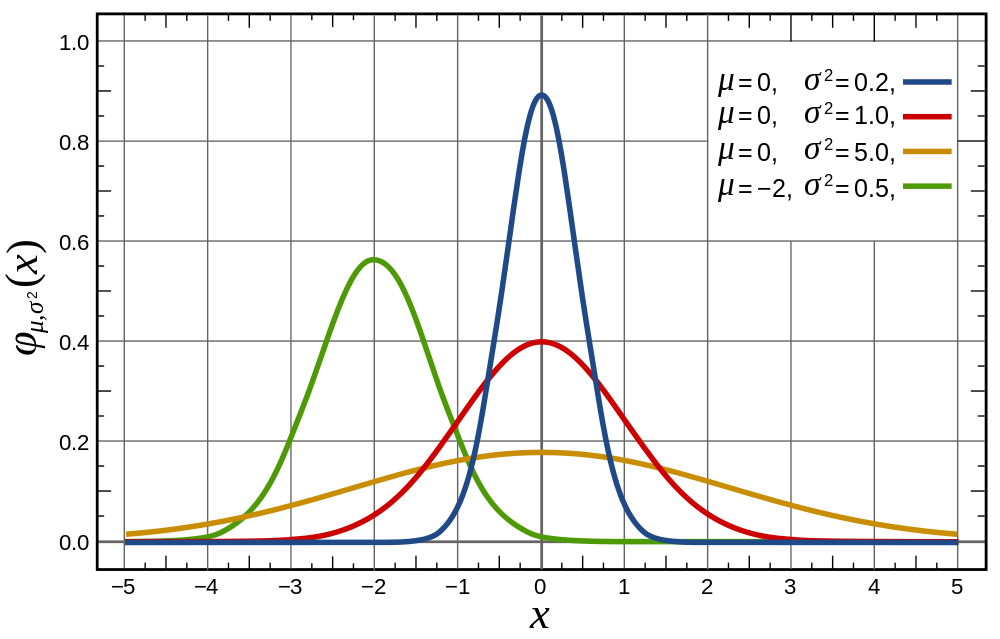
\includegraphics[scale=0.35]{figures/peak_1d}
  \caption[A 1-dimensional cross-section of Gaussian peaks.]
          {A 1-dimensional cross-section of Gaussian peaks.
           Each peak cross section may be characterized by its 
           position, as well as its width.  The peak as a whole
           has an intensity.  This image is in the
           public domain and was accessed at 
           \url{http://en.wikipedia.org/wiki/File:Normal_Distribution_PDF.svg}.}
  \label{peak_1d}
\end{figure}

\begin{figure}
  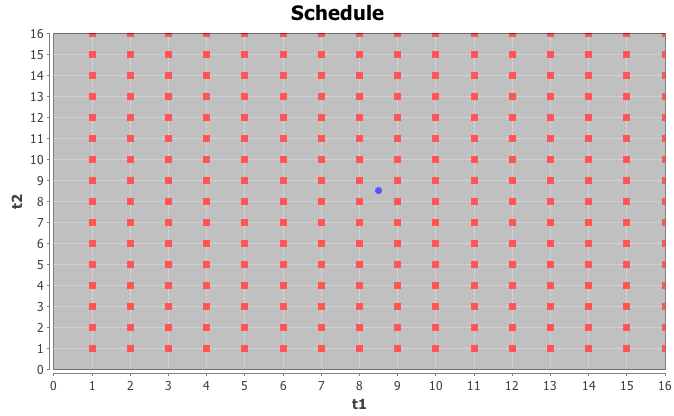
\includegraphics[scale=0.5]{figures/schedule_uniform}
  \caption[A uniform sample schedule.]
          {A uniform sample schedule.  The gaps between the points
           are constant.  The two axes represent the 
           variable time delays in the two indirect dimensions of a
           three-dimensional experiment.}
  \label{schedule_uniform}
\end{figure}

\begin{figure}
  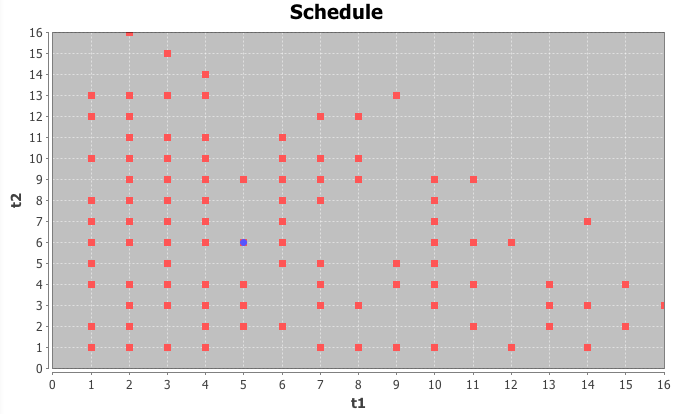
\includegraphics[scale=0.5]{figures/schedule_nonuniform}
  \caption[A non-uniform sample schedule.]
          {A non-uniform sample schedule.  The gaps between the points
           are not constant.  The two axes represent the 
           variable time delays in the two indirect dimensions of a
           three-dimensional experiment.}
  \label{schedule_nonuniform}
\end{figure}

\begin{figure}
  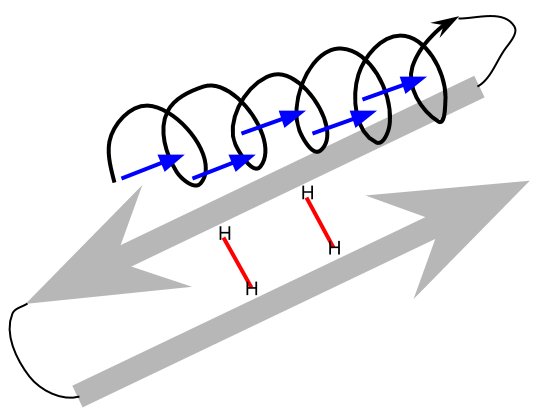
\includegraphics[scale=0.6]{figures/structure_restraints}
  \caption[Restraints are used to build a structural model.]
          {Restraints are used to build a structural model.
           Residual dipolar couplings give orientation constraints,
           and NOESY spectra give interatomic (H-H) distance constraints.}
  \label{structure_restraints}
\end{figure}

\begin{figure}
  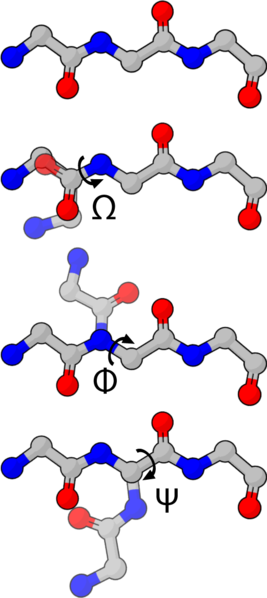
\includegraphics[scale=0.5]{figures/torsion_angles}
  \caption[Torsion angles provide structural information.]
          {Torsion angles provide structural information.
           A torsion angle is described by the positions of four
           atoms, and is the angle between two planes.  For protein
           structures, two key torsion angles are between the backbone
           atoms of each residue.
           This image is in the public domain, and was accessed
           from \url{http://en.wikipedia.org/wiki/File:Peptide_angles.png}.}
  \label{torsion_angles}
\end{figure}

% prevents a "! LaTeX Error: Too many unprocessed floats."
% see http://tex.stackexchange.com/a/46514/28358
\clearpage

\begin{figure}
  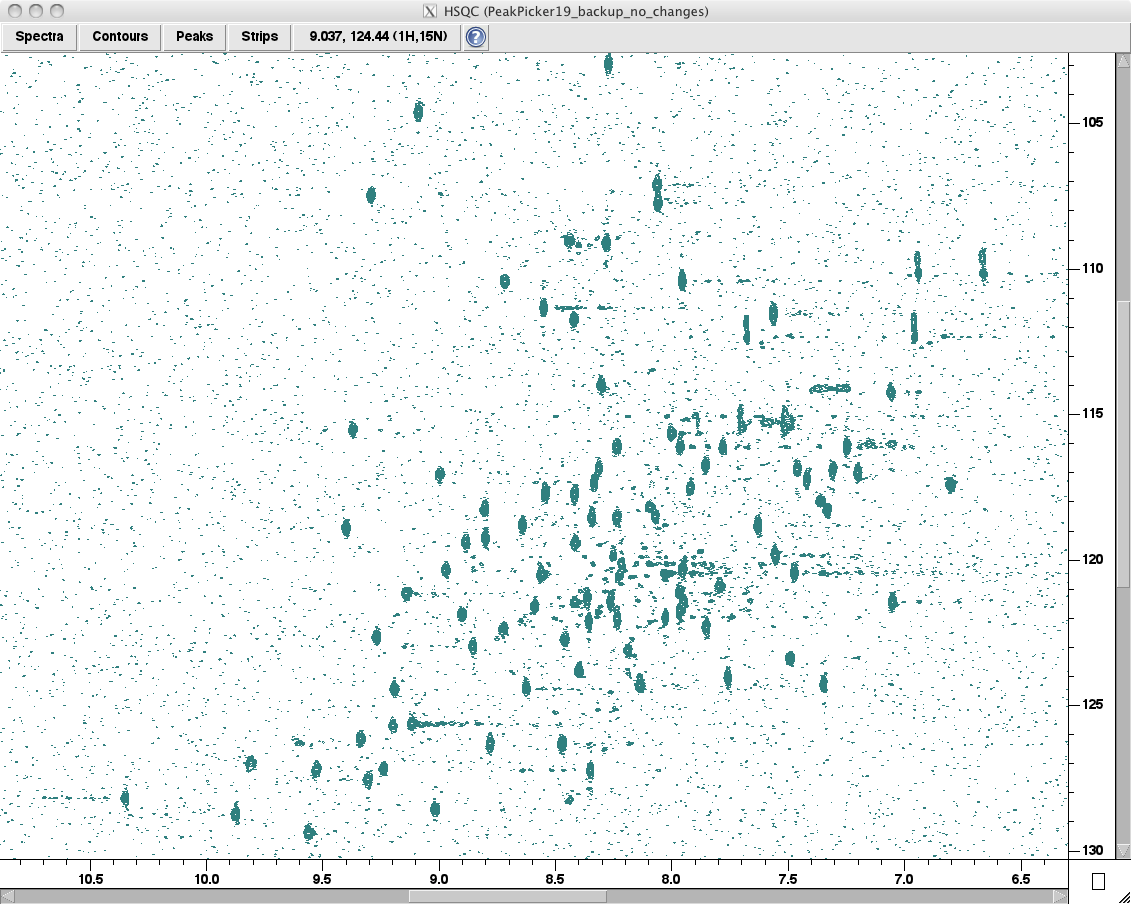
\includegraphics[scale=0.35]{figures/nhsqc}
  \caption[A frequency-domain NHSQC spectrum.]
          {A frequency-domain NHSQC spectrum. 
           The x- and y-axes are nitrogen and proton, respectively.}
  \label{nhsqc}
\end{figure}

\begin{figure}
  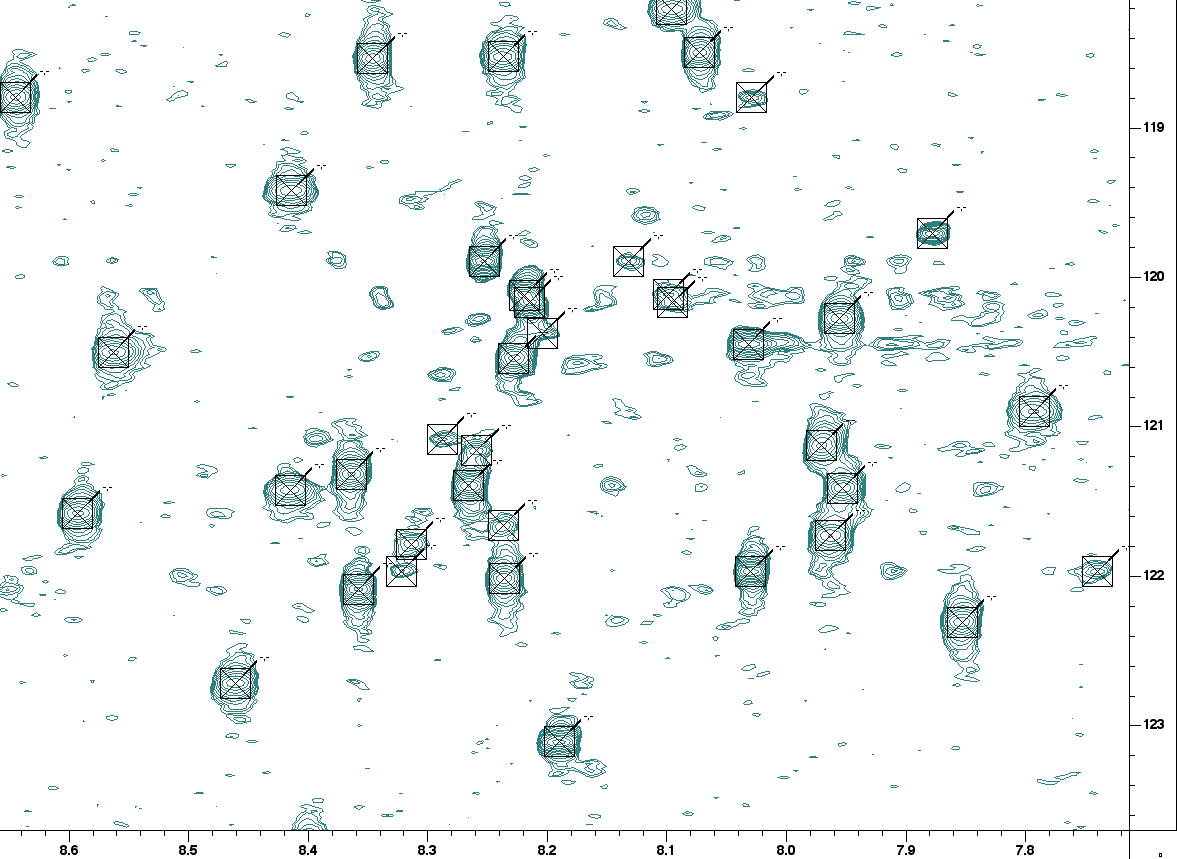
\includegraphics[scale=0.30]{figures/nhsqc_peaks}
  \caption[A peak picked NHSQC spectrum.]
          {A peak picked NHSQC spectrum. 
           Peaks are indicated by squares and crosses.}
  \label{nhsqc_peaks}
\end{figure}

\begin{figure}
  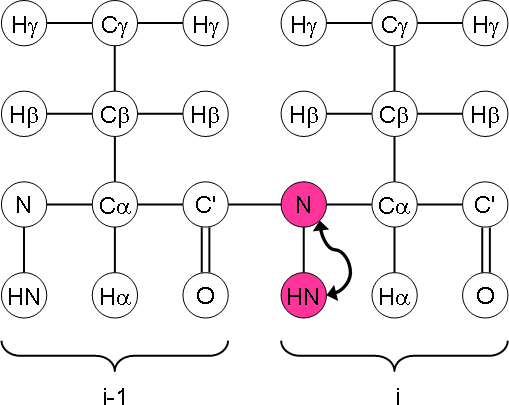
\includegraphics[scale=0.75]{figures/ccpn_nhsqc}
  \caption[The nuclei correlated by an NHSQC.]
          {The nuclei correlated by an NHSQC.
           This figure is reproduced from \url{http://www.protein-nmr.org.uk/}
           with the permission of Victoria Higman.}
  \label{ccpn_nhsqc}
\end{figure}

\begin{figure}
  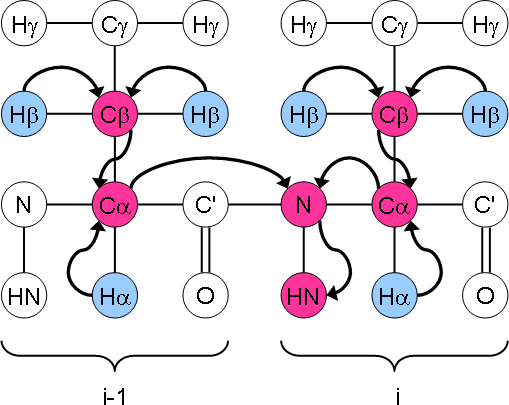
\includegraphics[scale=0.75]{figures/ccpn_hncacb}
  \caption[The nuclei correlated by an HNCACB.]
          {The nuclei correlated by an HNCACB.
           This figure is reproduced from \url{http://www.protein-nmr.org.uk/}
           with the permission of Victoria Higman.}
  \label{ccpn_hncacb}
\end{figure}

\begin{figure}
  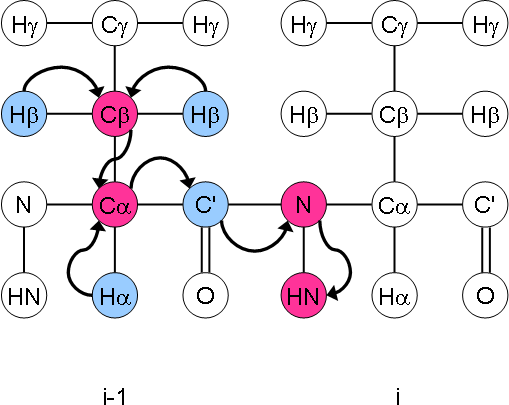
\includegraphics[scale=0.75]{figures/ccpn_cbcaconh}
  \caption[The nuclei correlated by a CBCA(CO)NH.]
          {The nuclei correlated by a CBCA(CO)NH.
           This figure is reproduced from \url{http://www.protein-nmr.org.uk/}
           with the permission of Victoria Higman.}
  \label{ccpn_cbcaconh}
\end{figure}

\begin{figure}
  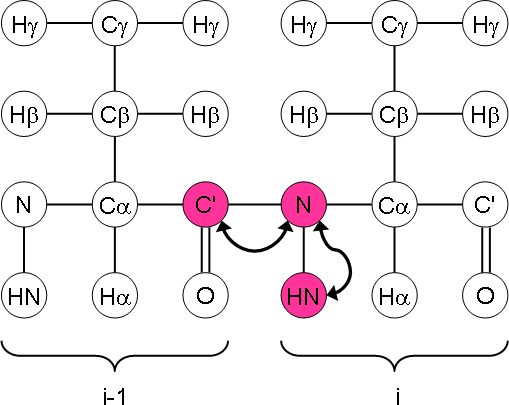
\includegraphics[scale=0.75]{figures/ccpn_hnco}
  \caption[The nuclei correlated by an HNCO.]
          {The nuclei correlated by an HNCO.
           This figure is reproduced from \url{http://www.protein-nmr.org.uk/}
           with the permission of Victoria Higman.}
  \label{ccpn_hnco}
\end{figure}

\begin{figure}
  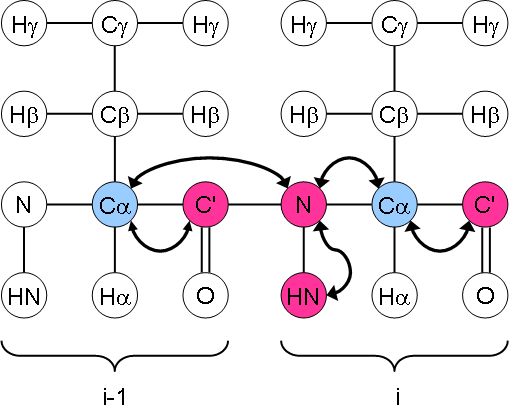
\includegraphics[scale=0.75]{figures/ccpn_hncaco}
  \caption[The nuclei correlated by an HN(CA)CO.]
          {The nuclei correlated by an HN(CA)CO.
           This figure is reproduced from \url{http://www.protein-nmr.org.uk/}
           with the permission of Victoria Higman.}
  \label{ccpn_hncaco}
\end{figure}

\begin{figure}
  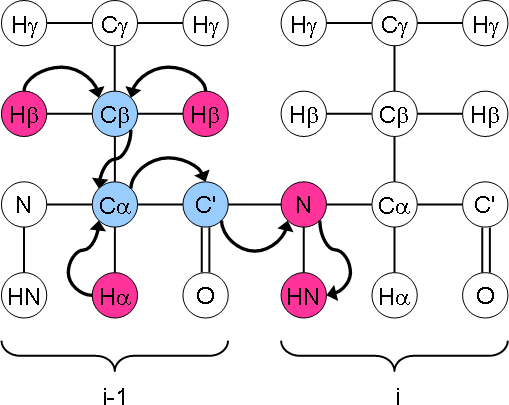
\includegraphics[scale=0.75]{figures/ccpn_hbhaconh}
  \caption[The nuclei correlated by an HBHA(CO)NH.]
          {The nuclei correlated by an HBHA(CO)NH.
           This figure is reproduced from \url{http://www.protein-nmr.org.uk/}
           with the permission of Victoria Higman.}
  \label{ccpn_hbhaconh}
\end{figure}

\begin{figure}
  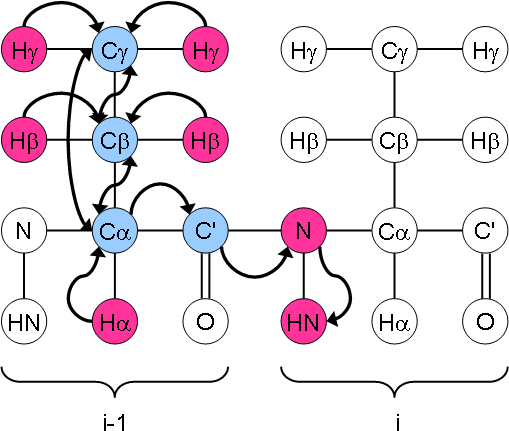
\includegraphics[scale=0.75]{figures/ccpn_hcconhtocsy}
  \caption[The nuclei correlated by an H(CCO)NH-TOCSY.]
          {The nuclei correlated by an H(CCO)NH-TOCSY.
           This figure is reproduced from \url{http://www.protein-nmr.org.uk/}
           with the permission of Victoria Higman.}
  \label{ccpn_hcconhtocsy}
\end{figure}

\begin{figure}
  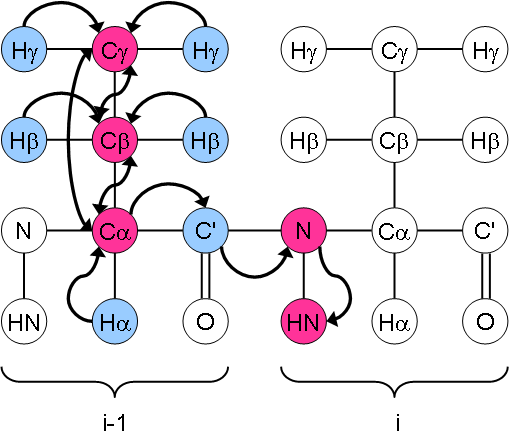
\includegraphics[scale=0.75]{figures/ccpn_cconhtocsy}
  \caption[The nuclei correlated by a C(CO)NH-TOCSY.]
          {The nuclei correlated by a C(CO)NH-TOCSY.
           This figure is reproduced from \url{http://www.protein-nmr.org.uk/}
           with the permission of Victoria Higman.}
  \label{ccpn_cconhtocsy}
\end{figure}

\begin{figure}
  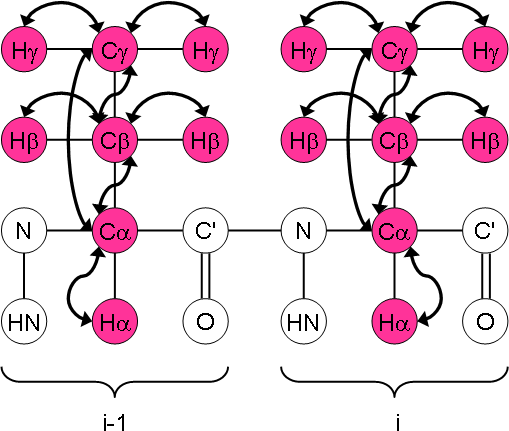
\includegraphics[scale=0.75]{figures/ccpn_hcchtocsy}
  \caption[The nuclei correlated by an HCCH-TOCSY.]
          {The nuclei correlated by an HCCH-TOCSY.
           This figure is reproduced from \url{http://www.protein-nmr.org.uk/}
           with the permission of Victoria Higman.}
  \label{ccpn_hcchtocsy}
\end{figure}

